\section{実験装置}
以下に実験に使用した装置およびスキャンした収穫物を示す.
3Dスキャナは非接触式でハンディタイプのArtec Leoを使用した.
スキャンした収穫物は, \figref{Fig:plant}に示すようなハウス内で栽培されているピーマン株である.
また, Blenderを用いてピーマンの3Dモデルから特性を計測した.
Blender利用するために使用したPCを\tabref{pc}に示す.

\begin{figure}[H]
   \centering
   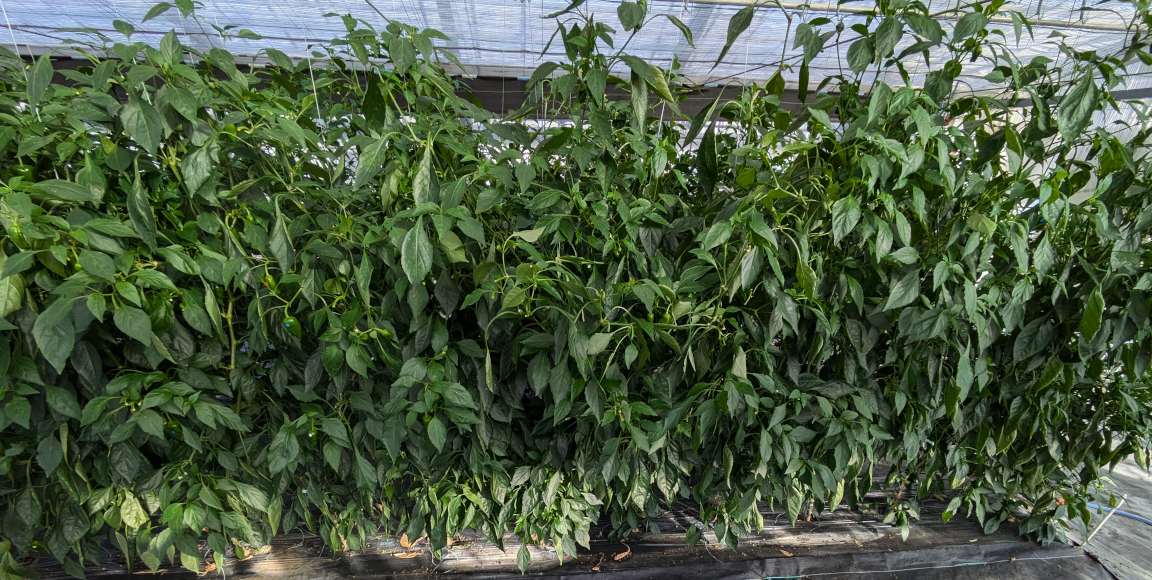
\includegraphics[width=110mm]{images/png/plant.png}
   \caption{Scanned crop}
   \label{Fig:plant}
\end{figure}

\begin{table}[H]
  \begin{center}
    \begin{tabular}{c|c}
      Processor & Spec\\ \hline\hline
      OS & Ubuntu20.04\\ \hline
      CPU & 11th Gen Intel(R) Core(TM) i7-1165G7 @ 2.80GHz × 8\\ \hline
      RAM & 15.2 GiB\\ \hline
    \end{tabular}
    \caption{PC Specifications}
    \label{Tab:pc}
  \end{center}
\end{table}